\section{Evaluation}
\label{sec:experiments}

We structure our evaluation around four research questions:

\noindent\textbf{RQ1:} How do kernels generated by \sys{} compare with
those produced by existing memory-based agents and with expert
implementations?

\noindent\textbf{RQ2:} Does a \sys improve kernel generation over providing expert source code directly?

\noindent\textbf{RQ3:} How well does \sys{} generalize to non-NVIDIA accelerators?

\noindent\textbf{RQ4:} How effectively can the induced skills be transfered to other operators and broader benchmarks?

\subsection{Setup}
\label{sec:exp-setup}

\paragraph{Platforms and languages.}
We evaluate on NVIDIA H100 PCIe (SM90), NVIDIA RTX PRO 6000 Blackwell (SM120), and Ascend 910B. On Nvidia, we use PyTorch 2.11.0+cu130, FlashInfer 0.6.11, TileLang 0.1.8, and FLA 0.5.0. FLA replaces FlashInfer as the GDN reference on SM120. On Ascend, we use CANN 9.1.0 and Torch-NPU 2.10.0. We build a separate skill library for each platform and record the verified architecture in each skill's scope. The target languages are CUDA C on NVIDIA and AscendC on Ascend.

\paragraph{Expert kernels and benchmarks.}
We select five expert kernels per platform, covering GEMM, Conv2d, FMHA, GDN, and Top-K. These operators are common in production, and their expert implementations contain a range of optimization techniques. Appendix~\ref{app:workload-detail} lists the workload shapes, data types, and reference implementations. The transfer targets and benchmark problems do not contribute to skill induction. We evaluate the transferability of the induced skills using 100 KernelBench Level~2 problems on NVIDIA GPUs and 100 problems from MultiKernelBench's Fusion category on Ascend NPUs.

\paragraph{Agents and budgets.}
We use Claude Code with Claude Opus 4.6 as the harness and LLM backbone  in \sys for offline skill induction and online kernel generation on both Nvidia and Ascend platforms. The online generation budget for these experiments is \$10 per workload; induction costs are reported separately. For operator transfer and benchmark evaluation on both platforms, we use Codex with DeepSeek-V4.1-Flash. Each transfer target has a two-hour wall-clock budget. Each problem in KernelBench or MultiKernelBench has a 30-minute wall-clock budget.
All reported costs are calculated using the corresponding model
providers' official API pricing.

\subsection{RQ1: Kernel Generation under induced Skill Library}
\label{sec:exp-induction}

We induce one library for each NVIDIA platform by the procedure of \autoref{sec:method-deopt} and \autoref{sec:method-extract}: walk each expert kernel backward under the checks, keep the reverse of every accepted step, and admit a lifted skill only once an agent handed that skill alone reproduces its effect on the deoptimized kernel.

As shown in \autoref{tab:roundtrip}, this procedure yields 52 admitted SkillCards on H100 and 36 on RTX PRO 6000 from the five expert kernels per platform listed in \autoref{tab:workload-detail}. The roundtrip admission rate is lower on H100: $72.2\%$ ($52/72$), compared with $80.0\%$ ($36/45$) on RTX PRO 6000. This difference is consistent with the more complex optimizations in the H100 experts, which use features such as distributed shared memory and warp-group tensor-core (WGMMA) instructions. Each SkillCard records the code and preconditions for applying an optimization, such as the layout requirements for WGMMA on H100. Induction is a one-time offline cost of \$131 on H100 and \$92 on RTX PRO 6000.


\begin{table}[h]
  \centering
  \small
  \setlength{\tabcolsep}{8pt}
  \begin{tabular}{@{}lccc@{}}
    \toprule
    \textbf{Platform} & \textbf{Skills in library} & \textbf{Roundtrip Admission} & \textbf{Induction cost (USD)} \\
    \midrule
    H100 (SM90)          & 52 & 52/72 & 131 \\
    RTX PRO 6000 (SM120) & 36 & 36/45 & 92 \\
    \bottomrule
  \end{tabular}
  \caption{The number of induced skills, roundtrip admission rate and induction cost of \sys{} on 2 Nvidia platforms across 5 expert kernels.}
  \label{tab:roundtrip}
\end{table}

\paragraph{What published memory-based agents reach on the same five kernels.}
Two systems already build a reusable memory for kernel optimization: AdaExplore~\citep{adaexplore}, which turns failures into rules and searches with MCTS, and AccelOpt~\citep{accelopt}, which keeps an LLM-summarized memory over the kernels it has generated. On the same five expert workloads, they reach $0.25\times$ and $0.54\times$ against the vendor reference and return no correct kernel at all on four and two of the ten workload--platform pairs; \sys{} reaches $1.12\times$ and is correct on all ten (\autoref{fig:cuda-bars}, absolute latencies in \autoref{tab:appendix-cuda-latencies}). Neither baseline converts more budget into a structurally different kernel, so we settle the comparison here and read the rest of the evaluation as \sys{} against the expert code it was induced from.

In \autoref{fig:cuda-bars}, a red $\times$ marks a workload with no correct kernel within the budget, and $\dagger$ marks the post-hoc adapter audit of AdaExplore's SM120 Conv2d kernel after excluding fallback wrappers.

\begin{figure*}[t]
\centering
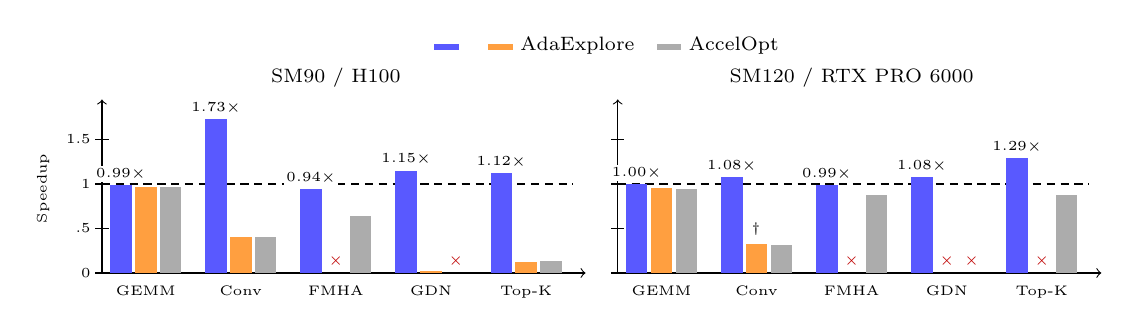
\begin{tikzpicture}[x=1.05cm,y=1.13cm]
  \node[anchor=south,font=\scriptsize] at (6.0,2.35) {%
    \tikz{\draw[fill=blue!65,draw=none] (0,0) rectangle (0.30,0.075);}~\sys{}\quad
    \tikz{\draw[fill=orange!75,draw=none] (0,0) rectangle (0.30,0.075);}~AdaExplore\quad
    \tikz{\draw[fill=gray!65,draw=none] (0,0) rectangle (0.30,0.075);}~AccelOpt};
\begin{scope}
  \draw[->] (-0.1,0) -- (5.75,0);
  \draw[->] (-0.1,0) -- (-0.1,1.95);
  \draw[densely dashed] (-0.1,1) -- (5.6,1);
  \draw (-0.18,0) -- (-0.02,0);
  \node[left,inner sep=1.5pt,font=\tiny] at (-0.18,0) {0};
  \draw (-0.18,0.5) -- (-0.02,0.5);
  \node[left,inner sep=1.5pt,font=\tiny] at (-0.18,0.5) {.5};
  \draw (-0.18,1) -- (-0.02,1);
  \node[left,inner sep=1.5pt,font=\tiny] at (-0.18,1) {1};
  \draw (-0.18,1.5) -- (-0.02,1.5);
  \node[left,inner sep=1.5pt,font=\tiny] at (-0.18,1.5) {1.5};
  \node[rotate=90,anchor=south,font=\tiny] at (-0.62,0.95) {Speedup};
  \node[anchor=south,font=\scriptsize] at (2.73,1.98) {SM90 / H100};
  \draw[fill=blue!65,draw=none] (0.0,0) rectangle ++(0.26,0.99);
  \draw[fill=orange!75,draw=none] (0.3,0) rectangle ++(0.26,0.97);
  \draw[fill=gray!65,draw=none] (0.6,0) rectangle ++(0.26,0.97);
  \node[anchor=south,inner sep=0.8pt,fill=white,font=\tiny] at (0.13,1.02) {$0.99{\times}$};
  \node[anchor=north,font=\tiny] at (0.43,-0.04) {GEMM};
  \draw[fill=blue!65,draw=none] (1.15,0) rectangle ++(0.26,1.73);
  \draw[fill=orange!75,draw=none] (1.45,0) rectangle ++(0.26,0.4);
  \draw[fill=gray!65,draw=none] (1.75,0) rectangle ++(0.26,0.41);
  \node[anchor=south,inner sep=0.8pt,fill=white,font=\tiny] at (1.2799999999999998,1.76) {$1.73{\times}$};
  \node[anchor=north,font=\tiny] at (1.5799999999999998,-0.04) {Conv};
  \draw[fill=blue!65,draw=none] (2.3,0) rectangle ++(0.26,0.94);
  \node[inner sep=0pt,font=\bfseries\tiny,red!75!black] at (2.7299999999999995,0.13) {$\times$};
  \draw[fill=gray!65,draw=none] (2.9,0) rectangle ++(0.26,0.64);
  \node[anchor=south,inner sep=0.8pt,fill=white,font=\tiny] at (2.4299999999999997,0.97) {$0.94{\times}$};
  \node[anchor=north,font=\tiny] at (2.73,-0.04) {FMHA};
  \draw[fill=blue!65,draw=none] (3.4499999999999997,0) rectangle ++(0.26,1.15);
  \draw[fill=orange!75,draw=none] (3.7499999999999996,0) rectangle ++(0.26,0.02);
  \node[inner sep=0pt,font=\bfseries\tiny,red!75!black] at (4.18,0.13) {$\times$};
  \node[anchor=south,inner sep=0.8pt,fill=white,font=\tiny] at (3.5799999999999996,1.18) {$1.15{\times}$};
  \node[anchor=north,font=\tiny] at (3.88,-0.04) {GDN};
  \draw[fill=blue!65,draw=none] (4.6,0) rectangle ++(0.26,1.12);
  \draw[fill=orange!75,draw=none] (4.8999999999999995,0) rectangle ++(0.26,0.12);
  \draw[fill=gray!65,draw=none] (5.199999999999999,0) rectangle ++(0.26,0.13);
  \node[anchor=south,inner sep=0.8pt,fill=white,font=\tiny] at (4.7299999999999995,1.1500000000000001) {$1.12{\times}$};
  \node[anchor=north,font=\tiny] at (5.029999999999999,-0.04) {Top-K};
\end{scope}
\begin{scope}[xshift=6.55cm]
\begin{scope}
  \draw[->] (-0.1,0) -- (5.75,0);
  \draw[->] (-0.1,0) -- (-0.1,1.95);
  \draw[densely dashed] (-0.1,1) -- (5.6,1);
  \draw (-0.18,0) -- (-0.02,0);
  \draw (-0.18,0.5) -- (-0.02,0.5);
  \draw (-0.18,1) -- (-0.02,1);
  \draw (-0.18,1.5) -- (-0.02,1.5);
  \node[anchor=south,font=\scriptsize] at (2.73,1.98) {SM120 / RTX PRO 6000};
  \draw[fill=blue!65,draw=none] (0.0,0) rectangle ++(0.26,1.0);
  \draw[fill=orange!75,draw=none] (0.3,0) rectangle ++(0.26,0.95);
  \draw[fill=gray!65,draw=none] (0.6,0) rectangle ++(0.26,0.94);
  \node[anchor=south,inner sep=0.8pt,fill=white,font=\tiny] at (0.13,1.03) {$1.00{\times}$};
  \node[anchor=north,font=\tiny] at (0.43,-0.04) {GEMM};
  \draw[fill=blue!65,draw=none] (1.15,0) rectangle ++(0.26,1.08);
  \draw[fill=orange!75,draw=none] (1.45,0) rectangle ++(0.26,0.33);
  \draw[fill=gray!65,draw=none] (1.75,0) rectangle ++(0.26,0.31);
  \node[anchor=south,inner sep=0.8pt,fill=white,font=\tiny] at (1.2799999999999998,1.11) {$1.08{\times}$};
  \node[anchor=south,inner sep=0.8pt,fill=white,font=\tiny] at (1.5799999999999998,0.36) {$^\dagger$};
  \node[anchor=north,font=\tiny] at (1.5799999999999998,-0.04) {Conv};
  \draw[fill=blue!65,draw=none] (2.3,0) rectangle ++(0.26,0.99);
  \node[inner sep=0pt,font=\bfseries\tiny,red!75!black] at (2.7299999999999995,0.13) {$\times$};
  \draw[fill=gray!65,draw=none] (2.9,0) rectangle ++(0.26,0.88);
  \node[anchor=south,inner sep=0.8pt,fill=white,font=\tiny] at (2.4299999999999997,1.02) {$0.99{\times}$};
  \node[anchor=north,font=\tiny] at (2.73,-0.04) {FMHA};
  \draw[fill=blue!65,draw=none] (3.4499999999999997,0) rectangle ++(0.26,1.08);
  \node[inner sep=0pt,font=\bfseries\tiny,red!75!black] at (3.8799999999999994,0.13) {$\times$};
  \node[inner sep=0pt,font=\bfseries\tiny,red!75!black] at (4.18,0.13) {$\times$};
  \node[anchor=south,inner sep=0.8pt,fill=white,font=\tiny] at (3.5799999999999996,1.11) {$1.08{\times}$};
  \node[anchor=north,font=\tiny] at (3.88,-0.04) {GDN};
  \draw[fill=blue!65,draw=none] (4.6,0) rectangle ++(0.26,1.29);
  \node[inner sep=0pt,font=\bfseries\tiny,red!75!black] at (5.029999999999999,0.13) {$\times$};
  \draw[fill=gray!65,draw=none] (5.199999999999999,0) rectangle ++(0.26,0.88);
  \node[anchor=south,inner sep=0.8pt,fill=white,font=\tiny] at (4.7299999999999995,1.32) {$1.29{\times}$};
  \node[anchor=north,font=\tiny] at (5.029999999999999,-0.04) {Top-K};
\end{scope}
\end{scope}
\end{tikzpicture}
\caption{Generated CUDA-kernel speedup over the platform-specific vendor reference. }
\label{fig:cuda-bars}
\end{figure*}

\subsection{RQ2: Expert Source versus Conditioned Skills}
\label{sec:exp-source-ablation}

We replace the conditioned skill library with expert kernel sources, keeping the rest of the setup fixed and allowing iterative refinement in both settings.

Generation from expert source is slower on all ten workload--platform pairs: $5.83$--$14.48\times$ on Conv2d and $37.43$--$105.18\times$ on GDN. The gap is smaller on GEMM and Top-K, at $1.12$--$1.48\times$. Per-workload latencies are reported in \autoref{tab:expert-source-ablation} (Appendix~\ref{app:tables}).

Even after repeated refinement, agents given expert source code often converge to simpler implementations that omit complex combinations of optimizations. On Conv2d, the agent reaches the appropriate tensor-core intrinsic but fails to combine it with the required shared-memory staging, swizzling, and pipelining. On SM90 GDN, it recovers the local \texttt{cumsum} transpose but omits the subsequent WGMMA, pipelining, and TMA optimizations. In both cases, the agent recovers an individual optimization while missing the intermediate code states needed to compose it with others. These results show that conditioned skills record these prerequisites and guide the agent in building the intermediate states needed for more complex optimizations. Roundtrip admission validates individual skills so that the LLM can tackle long-horizon optimization through small, verified steps, progressively implementing expert strategies while exploring alternative implementations.

\subsection{RQ3: Generalization beyond NVIDIA GPUs}
\label{sec:exp-ascend}

On accelerators with less publicly available kernel code, coding agents may have less prior knowledge of platform-specific optimizations. We use Ascend 910B to test whether \sys{} can obtain useful optimization knowledge from the same five expert kernels on a non-NVIDIA platform.
To this end, we induce the library from expert implementations in \texttt{torch-npu}, \texttt{cann-ops} and \texttt{vllm-ascend}, using the same five operator categories and workload shapes as on NVIDIA. Of 109 candidate skills, 67 pass roundtrip admission, yielding a rate of $61.5\%$, compared with $72.2\%$ on H100 and $80.0\%$ on RTX PRO 6000 (\autoref{tab:roundtrip}). Reaching a correct naive kernel on Ascend also requires more deoptimization steps than on NVIDIA. These difficulties are consistent with weaker model familiarity with Ascend programming, reflecting more limited coverage in pretraining data. The one-time offline induction cost is \$197.

We then generate AscendC kernels for the five workloads from naive implementations using the induced skills. The generated kernels outperform the expert baselines on all five workloads, with speedups of $1.048\times$--$1.496\times$ (\autoref{tab:ascend-compare}).

\begin{table}[h]
  \centering
  \small
  \setlength{\tabcolsep}{4.5pt}
  \begin{tabular}{@{}lccccc@{}}
    \toprule
    \textbf{Time ($\mu$s)} & \textbf{GEMM} & \textbf{Conv} & \textbf{FMHA} & \textbf{GDN} & \textbf{Top-K} \\
    \midrule
    \sys{}     & 424.2 & 17.74 & 6518.3 & 3393.4 & 15.48 \\
    Expert Baseline  & 444.6 & 26.54 & 7531.0 & 4764.4 & 19.83 \\
    \midrule
    Speedup    & $1.048\times$ & $1.496\times$ & $1.155\times$ & $1.404\times$ & $1.281\times$ \\
    \bottomrule
  \end{tabular}
  \caption{Generated AscendC-kernel speedup over the platform-specific vendor reference.}
  \label{tab:ascend-compare}
\end{table}

These results suggest that \sys{} can build on the small set of expert kernels available early in a new hardware platform's development. Engineers typically prioritize core operators such as GEMM, and guided deoptimization allows \sys{} to recover the hardware-specific knowledge in these implementations and reuse it to optimize other operators.

\subsection{RQ4: Transfer to New Operators and Benchmark Suites}
\label{sec:exp-transfer}

\paragraph{Operator transfer.}
On H100 and Ascend 910B, we evaluate transfer to five new operators: KDA, Sparse Attention, Top-P, Fused Add-RMSNorm, and GQA. None contributed to skill induction. We compare \sys{} with the Codex baseline, which receives no conditioned skills.

At the end of the budget, \sys{} retains faster kernels on every target where both settings produce valid kernels. Relative to Codex baseline, the geometric-mean speedup is $1.73\times$ over all five H100 targets and $1.41\times$ over the four Ascend targets with valid results from both settings. On the remaining Ascend target, Sparse Attention, \sys{} produces a valid kernel while Codex baseline fails. \autoref{fig:transfer-staircase} shows the optimization trajectories, and Appendix~\ref{app:transfer-axes} reports the corresponding token and cost trajectories. These results demonstrate that the skill libraries induced by \sys{} transfer to kernel-generation tasks for operators not used during induction.

\begin{figure*}[h]
\centering
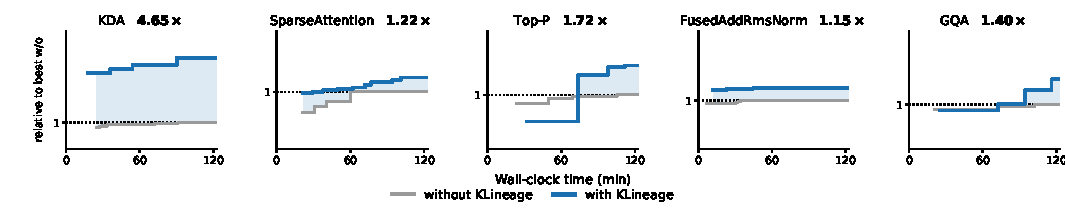
\includegraphics[width=\textwidth]{cuda_ab_time.pdf}
\par\vspace{1pt}
{\scriptsize (a) H100 (SM90)\par}
\vspace{4pt}
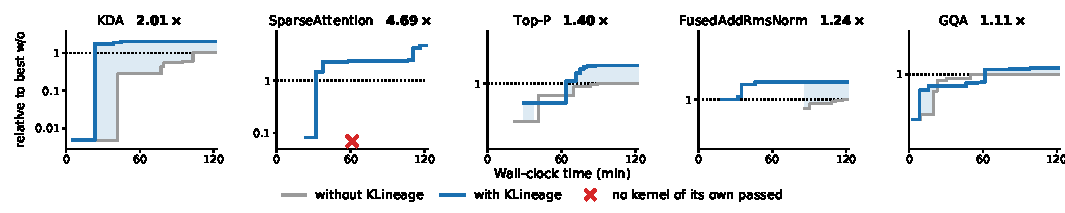
\includegraphics[width=\textwidth]{ascend_ab_time.pdf}
\par\vspace{1pt}
{\scriptsize (b) Ascend 910B\par}
\caption{\sys improve generation across the five transfer targets on H100 and Ascend 910B within two hours.}
\label{fig:transfer-staircase}
\end{figure*}

\paragraph{Optimizations recovered on Ascend.}
\autoref{tab:crossed} shows that \sys{} increases the total number of optimizations implemented across the five Ascend targets from 40 to 55, while preserving all optimizations found by the Codex baseline. Blue checkmarks indicate optimizations found only with \sys{}.

\begin{table*}[h]
\centering
\small
\setlength{\tabcolsep}{3.4pt}
\newcommand{\yes}{$\checkmark$}
\newcommand{\no}{\textcolor{black!35}{$\times$}}
\newcommand{\gain}{\textcolor{blue!70!black}{$\boldsymbol{\checkmark}$}}
\begin{tabular}{@{}l cc cc cc cc cc@{}}
\toprule
 & \multicolumn{2}{c}{\textbf{KDA}} & \multicolumn{2}{c}{\textbf{Top-P}}
 & \multicolumn{2}{c}{\textbf{GQA}} & \multicolumn{2}{c}{\textbf{Sparse Attn.}}
 & \multicolumn{2}{c}{\textbf{Add-RMSNorm}} \\
\cmidrule(lr){2-3}\cmidrule(lr){4-5}\cmidrule(lr){6-7}\cmidrule(lr){8-9}\cmidrule(lr){10-11}
\textbf{Optimization} & w/o & w/ & w/o & w/ & w/o & w/ & w/o & w/ & w/o & w/ \\
\midrule
Cube matmul for attention products   & \no & \no  & \no & \no   & \yes & \yes & \no & \gain & \no & \no   \\
Cube products split from Vector softmax & \no & \no & \no & \no & \yes & \yes & \no & \gain & \no & \no   \\
Work-aware launch partition          & \no & \no  & \no & \no   & \no & \gain & \no & \no   & \no & \gain \\
\addlinespace[1pt]
Two-slot / ping-pong staging         & \yes & \yes & \yes & \yes & \yes & \yes & \no & \gain & \yes & \yes \\
Prefetch ahead of compute            & \no & \gain & \no & \no   & \no & \no   & \no & \gain & \yes & \yes \\
Pack or transpose for downstream access & \no & \gain & \no & \no & \yes & \yes & \no & \no  & \no & \no   \\
Event-ordered overlap across streams  & \no & \no  & \no & \no   & \no & \gain & \no & \gain & \no & \no   \\
Workspace reuse across phases        & \no & \no  & \no & \no   & \no & \gain & \no & \gain & \no & \no   \\
L2 bypass for streaming writes       & \no & \no  & \no & \no   & \no & \no   & \no & \no   & \no & \gain \\
\addlinespace[1pt]
Row-max subtraction before exp       & \no & \no  & \no & \no   & \no & \gain & \yes & \yes & \no & \no   \\
GatherMask compaction of threshold band & \no & \no & \no & \gain & \no & \no  & \no & \no   & \no & \no   \\
\midrule
\multicolumn{11}{@{}l}{\textit{Nine further optimizations appear in both settings; the full audit is in \autoref{app:technique-matrix}.}} \\
\midrule
\textbf{Total (of 20)} & 7 & \textbf{9} & 8 & \textbf{9} & 10 & \textbf{14} & 7 & \textbf{13} & 8 & \textbf{10} \\
\bottomrule
\end{tabular}
\caption{\sys{} retains all 40 optimizations found without skills and adds 15 across the five Ascend transfer targets.}
\label{tab:crossed}
\end{table*}

\subsubsection{Generality to Broader Operators}
\label{sec:exp-kernelbench}

We test generality beyond the expert workloads on the $100$ Level~2 problems of KernelBench~\citep{kernelbench}, run on NVIDIA in CUDA and, as the Fusion category of MultiKernelBench~\citep{multikernelbench}, ported to AscendC on Ascend 910B. The two platforms therefore face the same $100$ problems rather than two different suites. Each platform's skill library remains unchanged, and none of these problems contributed to induction. Speedup is measured against \texttt{torch.compile} on NVIDIA and eager PyTorch on Ascend, then averaged over all valid solutions in each setting.

\autoref{tab:broader-operators} reports both evaluations. On NVIDIA, both settings produce correct kernels for all 100 problems; \sys{} raises mean speedup from $1.05\times$ to $1.32\times$ and the number of problems faster than \texttt{torch.compile} from 26 to 42. On Ascend, correctness rises from 68 to 100 problems, mean speedup from $0.63\times$ to $2.09\times$, and the number faster than eager from 22 to 93.

NVIDIA runs incur higher API costs because faster kernel execution and profiling allow more agent turns within the same wall-clock budget.

\begin{table}[ht]
  \centering
  \small
  \setlength{\tabcolsep}{6pt}
  \begin{tabular}{@{}lcccc@{}}
    \toprule
    \textbf{Method} & \textbf{Mean} & \textbf{Correct} & \textbf{Faster than} & \textbf{Cost} \\
                    & \textbf{speedup} & \textbf{(\%)}   & \textbf{reference (\%)}  & \textbf{(USD)} \\
    \midrule
    \multicolumn{5}{@{}l}{\textit{KernelBench Level 2 --- NVIDIA, CUDA}} \\
    without \sys{} & $1.05\times$ & 100 & 26 & 28.77 \\
    with \sys{} & $\mathbf{1.32\times}$ & 100 & \textbf{42} & 31.19 \\
    \midrule
    \multicolumn{5}{@{}l}{\textit{MultiKernelBench Fusion --- Ascend 910B, AscendC}} \\
    without \sys{} & $0.63\times$ & 68 & 22 & 21.92 \\
    with \sys{} & $\mathbf{2.09\times}$ & \textbf{100} & \textbf{93} & 24.05 \\
    \bottomrule
  \end{tabular}
  \caption{\sys{} improves performance on both broader operator benchmarks while producing correct kernels for all evaluated problems.}
  \label{tab:broader-operators}
\end{table}
